\documentclass{beamer}
\usepackage{graphicx,url}
\usepackage{amsmath}
\usepackage{amssymb}
\usepackage{xkeyval}

\usepackage{mytikz}

\usepackage{basics}
\usepackage{basics-slides}

\newcommand{\lf}{\mathit{LF}}
\newcommand{\kity}{\mathit{type}}

\renewcommand{\emph}[1]{\alert{#1}}

%\setbeamertemplate{headline}{\small\hfill\insertsection \hfill\hbox{}}

% building, browsing
% Mihnea can set up server for examples, tutorial as part of examples
% TODO: clean up urtheories, examples: only 2 prover examples fail (successful version is pushed)

\begin{document}

\title{MMT Tutorial, Part 1: \\ Designing Languages in MMT}
\author{Florian Rabe, Mihnea Iancu, Dennis M\"uller}
\institute{Jacobs University Bremen}
\date{CICM 2016}
\begin{frame}
    \titlepage 
\begin{center}
Bringing your notebook is recommended but not required.
\end{center}
\end{frame}


\section{Structure of the Tutorial}

\begin{myframe}{Overview}
\begin{enumerate}
 \item Brief introduction to MMT
 \item Download, install MMT and MMT IDE
 \item Design languages in MMT
   \begin{enumerate}
     \item LF as an example of a logical framework LF
     \item FOL as an example of a formal language
     \item algebraic theories as examples of domain knowledge
     \item module system for algebra
     \item design logics modularly
     \item implement logical frameworks modularly
   \end{enumerate}
 \end{enumerate}
\end{myframe}

\begin{myframe}{Further Resources}
\begin{itemize}
  \item MMT homepage: \url{http://uniformal.github.io/}
  \item Introductory articles: \url{http://uniformal.github.io/doc/philosophy/intros.html}
  \item Publications: \url{http://uniformal.github.io/doc/philosophy/papers.html}
  \item Sources:  \url{http://uniformal.github.io/MMT}
  \item API documentation:  \url{http://uniformal.github.io/apidoc}
\end{itemize}
\end{myframe}

\section{Motivation of MMT}

\begin{myframe}{Language-Independence}
\begin{block}{MMT = meta-meta-theory/tool}
\centering
a universal framework for the \\ formal representation of all knowledge and its semantics \\ in math, logic, and computer science
\end{block}

\begin{itemize}
	\item Avoid fixing languages wherever possible 
	\item Use formal meta-languages for defining languages \ldots
	\item \ldots and avoid fixing even the meta-languages. 
\end{itemize}
\lec{Obtain (meta-)language-independent results}

\begin{center}
\begin{tabular}{|p{2cm}|p{2cm}|p{2cm}|p{2cm}|}
\hline
Mathematics      & Formalization            & Logical Framework    & Language-Independence \\
\hline
\hline
\multicolumn{3}{|c|}{} & meta-meta-framework\\\cline{3-4}
\multicolumn{2}{|c|}{} & \multicolumn{2}{c|}{meta-language}\\\cline{2-4}
                      & \multicolumn{3}{c|}{language (logics, DSLs, etc.)}\\\hline
\multicolumn{4}{|c|}{domain knowledge} \\
\hline
\end{tabular}
\end{center}
\end{myframe}

\begin{myframe}{Subsume All Paradigms of Knowledge Representation}
\begin{itemize}
\item Conceptualization: \hlE{identifiers and their properties}
\item Narration:
  \hlE{human-oriented, informal-but-rigorous}
\item Deduction:
  \hlE{machine-verificable, formal}
\item Computation: \hlE{executable, algorithmic}
\item Tabulation:
  \hlE{databases, queryable}
\end{itemize}

\vspace{-.5em}
\begin{center}
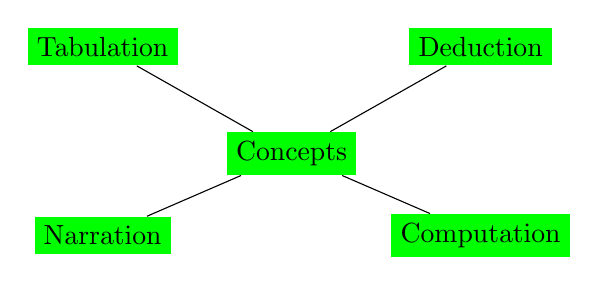
\begin{tikzpicture}[scale=.8]
\node[fill=green] (Cn)  at (0,1.3)   {Concepts};
\node[fill=green] (D)  at (3,3)   {Deduction};
\node[fill=green] (T)  at (-3,3)   {Tabulation};
\node[fill=green] (Cm)  at (3,0)   {Computation};
\node[fill=green] (N)  at (-3,0)   {Narration};

\draw[-] (Cn) -- (D);
\draw[-] (Cn) -- (T);
\draw[-] (Cn) -- (Cm);
\draw[-] (Cn) -- (N);
\end{tikzpicture}
\end{center}
\end{myframe}

\begin{myframe}{Design Principles}
\begin{blockitems}{Separation of concerns between}
  \item language development
    \lec{logical primitives, rules}
  \item knowledge management
 	\lec{e.g., search, change management}
  \item verification
 	\lec{e.g., type checking, theorem prover}
  \item application development
 	\lec{e.g., IDE, proof assistant}
\end{blockitems}

\begin{blockitems}{Universal language}
\item few primitives $\ldots$
\item that unify different domain concepts
\end{blockitems}

\begin{blockitems}{Language-Independent Implementations}
\item possible for surprisingly many results
\item yields rapid prototyping for logic systems
\end{blockitems}
\end{myframe}

%\begin{myframe}{Some Principles}
%	\begin{itemize}
%		\item judgments as types, proofs as terms
%		\lec{unifies expressions and derivations}
%		\item higher-order abstract syntax
%		\lec{unifies operators and binders}
%		\item category of theories and theory morphisms
%		\begin{itemize}
%			\item languages as theories
%		\lec{unifies logical theories, logics, foundations}
%			\item relations as theory morphisms
%		\lec{unifies modularity, intepretations, representation theorems}
%		\end{itemize}
%		\item institution-style abstract model theory
%		 \lec{uniform abstract concepts}
%		\item models as morphisms (categorical logic)
%		\lec{unifies models and translations and semantic interpretations}
%	\end{itemize}
%\end{myframe}

%\begin{blockenum}{Design Cycle}
%	\item Choose a typical problem
%	\item Survey and analyze the existing solutions
%	\item Differentiate between \emph{foundation-specific} and \emph{foundation-independent} concepts/problems/solutions
%	\item Integrate the foundation-independent aspects into MMT
%	\item Define interfaces to supply the foundation-specific aspects
%\end{blockenum}

\begin{myframe}{Language-Independent Results So Far}
\begin{blockitems}{Knowledge Management}
		\item Change management
		  \lec{recheck only if affected}
		\item Project management
		  \lec{indexing, hosting}
		\item Extensible build system
		  \lec{presentation, import/export, \ldots}
		\item Search, querying
		  \lec{substitution-tree and relational index}
		\item Browser
		  \lec{interactive web browser}
		\item Editing
		  \lec{IDE-like graphical interface}
\end{blockitems}

\begin{blockitems}{Logical Results}
		\item Module system
		  \lec{modularity transparent to foundation developer}
		\item Concrete/abstract syntax
		  \lec{notation-based parsing/presentation}
%		\item Interpreted symbols, literals
%		  \lec{external model/implementation reflected into \mmt}
		\item Type reconstruction
		  \lec{foundation plugin supplies only core rules}
		\item Simplification
		  \lec{rule-based, integrated with type reconstruction}
		\item Anticipated: Theorem proving, code generation, stateful computation
\end{blockitems}
\end{myframe}

\begin{myframe}{Meta-Hierarchy}
 \begin{center}
 \framebox{
 \begin{tikzpicture}
 \node (MMT) at (3,1.5) {MMT};
 \node (L) at (2,0.5) {LF};
 \node (Lx) at (4,0.5) {LF+X};
 \draw[arrow](MMT) -- (L);
 \draw[arrow](MMT) -- (Lx);

 \draw[fill=red!60] (2,-.5) ellipse (3.2cm and .6cm);
 \node[color=red] at (-3.3,-.5) {LATIN logic library};
 \node at (2,-.7) {\ldots};

 \draw[fill=blue!60] (0,-2.25) ellipse (1.9cm and .8cm);

 \node (H) at (0,-.5) {HOL Light};
 \node[color=blue!80] at (-3.5,-2) {HOL Light library};
 \node (B) at (-1,-2) {Bool};
 \node (A) at (1,-2) {Arith};
 \node (E) at (0,-2.5) {\ldots};
 \draw[arrow](L) -- (H);
 \draw[arrow](H) -- (B);
 \draw[arrow](H) -- (A);
 \draw[arrow](B) -- (A);

 \draw[fill=olive] (4,-2.25) ellipse (1.9cm and .8cm);

 \node (M) at (4,-.5) {Mizar};
 \node[color=olive] at (-3.3,-2.5) {Mizar library};
 \node (B') at (3,-2) {XBoole};
 \node (A') at (5,-2) {XReal};
 \node (E') at (4,-2.5) {\ldots};

 \node (A) at (1,-2) {Arith};
 \node (E) at (0,-2.5) {\ldots};
 \draw[arrow](L) -- (M);
 \draw[arrow](M) -- (B');
 \draw[arrow](M) -- (A');
 \draw[arrow](B') -- (A');
 \end{tikzpicture}
 }
 \end{center}
\end{myframe}


\end{document}

